\documentclass{article}

\usepackage{nameref}
\usepackage{graphicx}
\usepackage{hyperref}

\title{MLM Project}
\author{Mavin Martin\\
Scientific Computing \& Imaging}

\setlength{\parindent}{0pt}
\begin{document}
\maketitle
\section{Viewing Neuron Cell inside of SCIRun 4}
\label{viewing_neuron_cell}
To be able to visualize neuron voltages inside of SCIRun, you would need to create several files. where $n$ is the number of points you want to display.\\

\textbf{my\_file.pts}\\
\begin{math}
	\begin{array}{l}
	x_1,y_1,z_1\\
	x_2,y_2,z_2\\
	x_{n-1},y_{n-1},z_{n-1}\\
	x_n,y_n,z_n
	\end{array}
\end{math}\\\\


$x_n$ in the above example is the number of points you want to display.\\

\textbf{my\_file.edge}\\
\begin{math}
	\begin{array}{lll}
	1 & 2 & //pt_1-pt_2\\
	3 & 2 & //pt_3-pt_2\\
	n & 2 & //pt_n-pt_2
	\end{array}
\end{math}\\\\

The above example creates the following edges between two points in the \textbf{my\_file.pts} file.  Be sure not to place comments in the edge file, they are here for understanding only.\\

To visualize the points inside SCIRun, create the following modules.

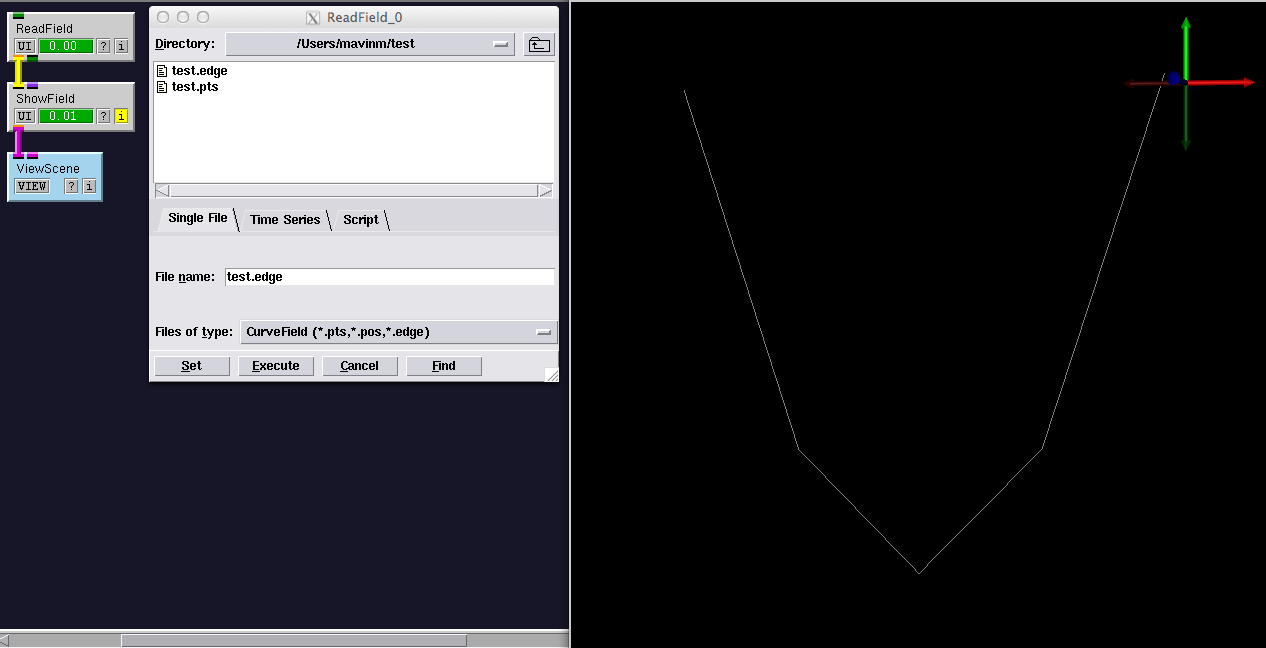
\includegraphics[width=\textwidth]{images/pt_edge_example.png}\\

Be sure that the \textbf{ReadField} file type is \textit{CurveField}.  I have plotted a parabola as an example.

\section{Color Coding Neuron Cells}

To color code the neuron cells, it requires an additional step to the section \nameref{viewing_neuron_cell}.\\

For the practical use, you have to map each point an isovalue.  To do this, create a matrix of values.  In my example, we will make every row a time instance and every column a map to each point.  It is important that the number of values you have match the number of points in the \textbf{my\_file.pts}.\\

\textbf{voltages.txt}\\
\begin{math}
	\begin{array}{lllll}
	I_{(1,1)} & I_{(1,2)} & ... & I_{(1,n-1)} & I_{(1,n)}\\
	I_{(2,1)} & I_{(2,2)} & ... & I_{(2,n-1)} & I_{(2,n)}\\
	... & ... & ... & ... & ...\\
	I_{(t-1,1)} & I_{(t-1,2)} & ... & I_{(t-1,n-1)} & I_{(t-1,n)}\\
	I_{(t,1)} & I_{(t,2)} & ... & I_{(t,n-1)} & I_{(t,n)}\\
	\end{array}
\end{math}\\\\

where in the variable $I_{(t,n)}$, $I$ is the intensity value, $t$ is the time instance, and $n$ is the point in \textbf{my\_file.pts} that you want to map the isovalues to.

To get the data into SCIRun, you must now create another file that's a nrrd format(\url{http://teem.sourceforge.net/nrrd/}).  You can look at the source documentation for more advanced data, for mapping a matrix to a point file, you would simply copy these lines into the following file.\\

\textbf{voltages.nhdr}\\
\begin{itshape}
NRRD0001\\
\# Author : YOURNAME\\
\# Formatting of data\\
type: float\\
\# 2-Dimensions\\
dimension: 2\\
\# Number of elements in X,Y\\
sizes: N T\\
\# Linked Source File\\
data file: FILENAME\\
\# Formatting of data file\\
encoding: ascii
\end{itshape}\\

where in the file you will change \textit{YOURNAME} to your preferred author name, \textit{N} to the number of points in \textbf{my\_file.pts}, \textit{T} to the number of time instances, and \textit{FILENAME} to the full path to the matrix file.\\

Finally, to load the correct modules into SCIRun add to the modules you've created in \nameref{viewing_neuron_cell}.\\

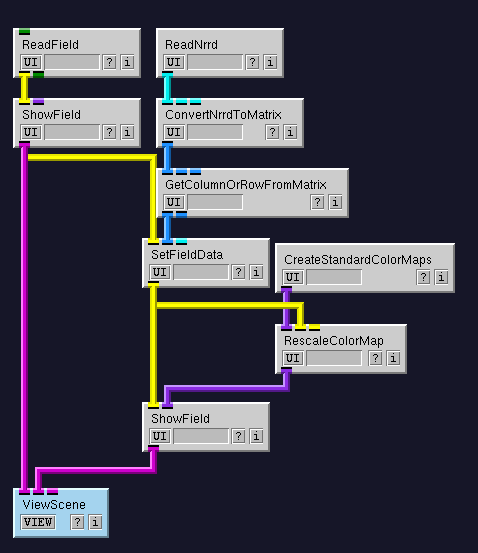
\includegraphics[width=0.8\textwidth]{images/voltage_example.png}
\end{document}
